\chapter{Grundlagen}

Dieses Kapitel stellt die Grundlagen der Arbeit dar. Diese bestehen aus den verschiedenen Service-Modellen des Cloud Computings, welche definiert und voneinander abgegrenzt werden. Darauf folgt ein Abschnitt, der die nötigen Tools der Anwendungen sowie weitere dieser Art vorstellt.

\section{Service-Modelle}

Einer der Vorreiter des Cloud Computing ist John McCarthy, der in einer Rede am Massachusetts Institute of Technology (MIT) 1961 den Begriff des Utility Computings prägte. In dieser Rede ging er davon aus, dass in der Zukunft Rechenleistung ebenso wie das Telefonsystem als öffentliche Versorgung organisiert sind. Vergleichbar soll diese Versorgung dann mit Wasser, Strom und Gas sein. Entsprechend haben sich bis heute einige große Cloud-Anbieter wie \ac{AWS}, Google Cloud Platform oder Microsoft Azure entwickelt. Deren Geschäftsmodell begann damit, dass sie ihre überschüssige Rechenleistung als öffentlichen Dienst angeboten haben. Dies wird aber mehr und mehr zum Kerngeschäft dieser Unternehmen. \autocite{buyya2013mastering}

Allgemein lässt sich die Cloud in verschiedene Service-Modelle wie \ac{IaaS}, \ac{PaaS}, \ac{FaaS}, \ac{BaaS} oder \ac{SaaS} unterteilen. Die Definition, Abgrenzung und Einordnung dieser Modelle und Begriffe wird in verschiedener Literatur \autocite{jiang2020overview}\autocite{kumar2019serverless}\autocite{dahunsi2021commercial} behandelt. Zusätzlich ist noch zu erwähnen, dass schlussendlich alles als Dienst angeboten werden kann. So hat sich \ac{XaaS} etabliert. Weitere Beispiele für die solche Cloud-Dienste angeboten werden, sind AI as a Service, API as a Service, Analytics as a Service oder Knowledge as a Service.

\subsection{\acl{IaaS}}

Bei \acf{IaaS} stellt der Anbieter dem Kunden Infrastrukturelemente für eine Software bereit. Beispiele für solche Elemente sind virtuelle Maschinen, Server, Speicherplätze und Netzwerke. Bei \ac{AWS} gibt es für die genannten Beispiele die \ac{EC2}. In der Google Cloud Platform ist es die Compute Engine. In der Regel zahlt der Kunde nur für das, was er in einem bestimmten Zeitabschnitt tatsächlich genutzt hat.

Der Vorteil liegt darin, dass auf Grund der Vertragsstruktur jederzeit neue Elemente hinuzugebucht oder gekündigt werden können. Das macht \acl{IaaS} flexibler und skalierbarer gegenüber dem herkömmlichen Ansatz, Server für eine bestimmte Vertragslaufzeit zu mieten oder gar vollständig zu erwerben. Auch soll ein Anreiz sein, dass dies gegenüber dem herkömmlichen Ansatz kostengünstiger ist.

Nachteilig ist allerdings, dass die Server in einem externen Rechenzentrum liegen und somit die Sicherheit nicht in der eigenen Hand liegt, was eine gängige Herausforderung beim Cloud Computing darstellt. So wie bei allen weiteren Service-Modellen benötigt der Kunde eine stetige Internetverbindung zum Server, selbst wenn es sich nur um eine firmeninterne Anwendung handelt.

\subsection{\acl{PaaS}}

\acf{PaaS} baut auf \acl{IaaS} auf und bietet zusätzlich eine Entwicklungsplattform mit Tools zum Entwickeln als Dienst an. Beispiele für \ac{PaaS} sind \ac{AWS} Elastic Beanstalk, Google App Engine und Heroku.

Die Vor- und Nachteile von \acl{IaaS} treffen hier auch zu. Zusätzlich ist ein Vorteil, dass der Kunde sich nicht mehr selbst um die Hard- und Software kümmern muss, sondern sich lediglich auf die Entwicklung von Software-Produkten fokussieren kann. Der Anbieter selbst wickelt die Wartung und Pflege ab. Ein Nachteil ist, dass Entwickler keinen Einfluss auf die Umgebung selbst nehmen können, falls sie diese im Zweifelsfall verändern müssen.

\subsection{\acl{FaaS}}

Die Domänenlogik einer Anwendung kann mittels \acf{FaaS} abgebildet werden. Es handelt sich um Funktionen, die mit Parametern über Trigger aufgerufen werden können. Solch eine Funktion liegt nicht auf eigenen Servern, sondern beim jeweiligen Anbieter. Die Abgrenzung zu \ac{PaaS} ist, dass es sich hierbei nur um Funktionen handelt, während es sich bei \ac{PaaS} um eine ganze Anwendung handelt. Somit entsteht bei \ac{FaaS} die Anwendung dadurch, dass beispielsweise ein API-Gateway die Funktion aufruft. Beispiele für \ac{FaaS} sind \ac{AWS} Lambda, Google Cloud Functions, Azure Functions oder IBM OpenWhisk.

Ein Vorteil von \ac{FaaS} ist die Skalierbarkeit, die vom Anbieter selbst verwaltet wird. Außerdem ist \ac{FaaS} plattformunabhängig, so dass in jeder angebotenen Programmiersprache entwickelt werden kann. Dadurch, dass nur das bezahlt wird, was auch genutzt wird, ist \ac{FaaS} in der Regel kostengünstiger als dauerhaft einen Server laufen zu lassen. Des Weiteren bieten die meisten Anbieter auch schon direkt Anbindungen zum Logging und Monitoring ein, was die Überwachung der Funktionen vereinfacht.

Ein Nachteil von \ac{FaaS} sind beispielsweise die Startzeit von Funktionen. Je größer der Speicherplatz einer Funktion ist, desto länger dauert die Startzeit von Funktionen. Möchte der Entwickler keine Aufwärmzeit, muss für Provisioned Concurrency bezahlt werden. Ein weiterer Nachteil ist, dass Funktionen eine maximale Ausführungsdauer haben, welche von Cloud-Anbieter variiert. Für größere Workloads muss dann eine Alternative gefunden werden.

\subsection{\acl{BaaS}}

\acf{BaaS}, auch \ac{MBaaS} genannt, wenn es speziell um mobile Applikationen geht, zielt darauf ab, dass Entwickler im Backend auf bereits bestehende Schnittstellen zugreifen können, um gängige Herausforderungen mit möglichst wenig Quellcode lösen zu können. Die folgende Auflistung gibt eine erste Übersicht über die oftmals schon vorhandenen Schnittstellen:
\begin{itemize}
  \item Authentifizierung- und Autorisierung
  \item Hosting
  \item Datenbank-Management
  \item Push Notifications
  \item Storage
  \item Analytics
  \item Geo-Dienste
  \item Maschinelles Lernen
\end{itemize}

Der Fokus wandert damit vom Backend hin zum Frontend, welches die Schnittstellen aufruft. Dennoch gibt es auch im Backend Quellcode, der geschrieben werden muss. Dies erfolgt wieder über Funktionen durch \ac{FaaS}. \ac{AWS} Amplify und Firebase lassen sich in die Kategorie der \ac{BaaS} eingliedern. Wird \ac{BaaS} mit \ac{FaaS} kombiniert, spricht man nach Mike Roberts auch von Serverless \autocite{brandon2017serverless}.

Die Vor- und Nachteile sind nahezu deckungsgleich mit denen von \ac{FaaS}. Es lässt sich noch hinzufügen, dass der Vendor lock-in bei \ac{BaaS} sich nochmal vergrößert, da viele verschiedene Dienste eines einzelnen Anbieters genutzt werden. Außerdem kann das Debugging und Monitoring auf Grund verschiedener Dienste komplexer als in üblichen Anwendungen werden.

\subsection{\acl{SaaS}}

\ac{SaaS} ist die gesamte Applikation als Dienst für den Endnutzer. Meistens ist eine Software dieser Art über ein oftmals monatliches Abonnement zu erhalten. Beispiels für Proukte dieser Art sind Slack, Microsoft 365, Salesforce oder Atlassian Jira.

Der Vorteil bei \ac{SaaS} ist, dass nicht die gesamte Software gekauft und bereitgestellt werden muss. Außerdem liefert der Hersteller regelmäßige Updates. Der Kunde muss sich also in der Regel nur noch um die Konfiguration der Anwendung selbst kümmern, während der Rest vollständig übernommen wird. Nachteilig ist damit allerdings auch, dass der Nutzer kaum Kontrolle über das Produkt hat. Des Weiteren liegen die Daten auch hier wieder auf einem externen Rechenzentrum, was auf Grund von Datensicherheit und der Datenschutz-Grundverordnung eine Hürde darstellt.

\subsection{Abgrenzung der Begriffe}

\begin{table}[h]
  \caption{Vergleich von Service-Modellen \autocite{jiang2020overview}}
  \label{Kap2:ServiceModelleVergleich}
  \renewcommand{\arraystretch}{1.2}
  \centering
  \sffamily
  \begin{footnotesize}
    \begin{tabular}{l l l l l}
    \toprule
    & \textbf{\ac{IaaS}} & \textbf{\ac{PaaS}} & \textbf{\ac{FaaS}} & \textbf{\ac{SaaS}}\\
    \midrule
    \textit{Entwicklungseffizienz} & Gering	&	Mittel	& Hoch & Hoch\\
    \textit{Skalierbarkeit} & Gering	&	Mittel & Hoch & Hoch\\
    \textit{Wartung} &	Gering	&	Hoch & Hoch & Hoch\\
    \textit{Kosten}	&	Hoch		&	Hoch & Gering & Hoch\\
    \textit{Anwender}	&	Administrator		&	Entwickler & Entwickler & Anwender\\
    \bottomrule
    \end{tabular}
  \end{footnotesize}
  \rmfamily
\end{table}

\autoref{Kap2:ServiceModelleVergleich} vergleicht \ac{IaaS}, \ac{PaaS}, \ac{FaaS}, damit implizit auch \ac{BaaS}, und \ac{SaaS} anhand den Kriterien Entwicklungseffizienz, Skalierbarkeit, Wartung, Kosten und den Anwendern.

Von links nach rechts nimmt dabei der Fokus auf die Business-Logik zu. Während bei \ac{IaaS} nur Infrastrukturelemente bereitgestellt werden, wird bei \ac{SaaS} die ganze Anwendung bereitgestellt. Dem entsprechend nimmt auch die Abstraktion von links nach rechts zu. Folglich nimmt die Flexibilität ab, da der Anwender bei \ac{SaaS} höchstens noch die Anwendung konfigurieren kann. Zwischen \ac{PaaS} und \ac{SaaS} hat \ac{FaaS} den Vorteil, dass dieser Dienst noch für Entwickler gedacht ist und damit flexibel genug ist, um Anwendungen aufzubauen. Dieser Vorteil trifft entsprechend auch auf \ac{BaaS} zu. \ac{FaaS} und \ac{BaaS} stellen alle nötigen Ressourcen exklusive des Anwendungslogik zur Verfügung.

\begin{figure}[h]
  \centering
  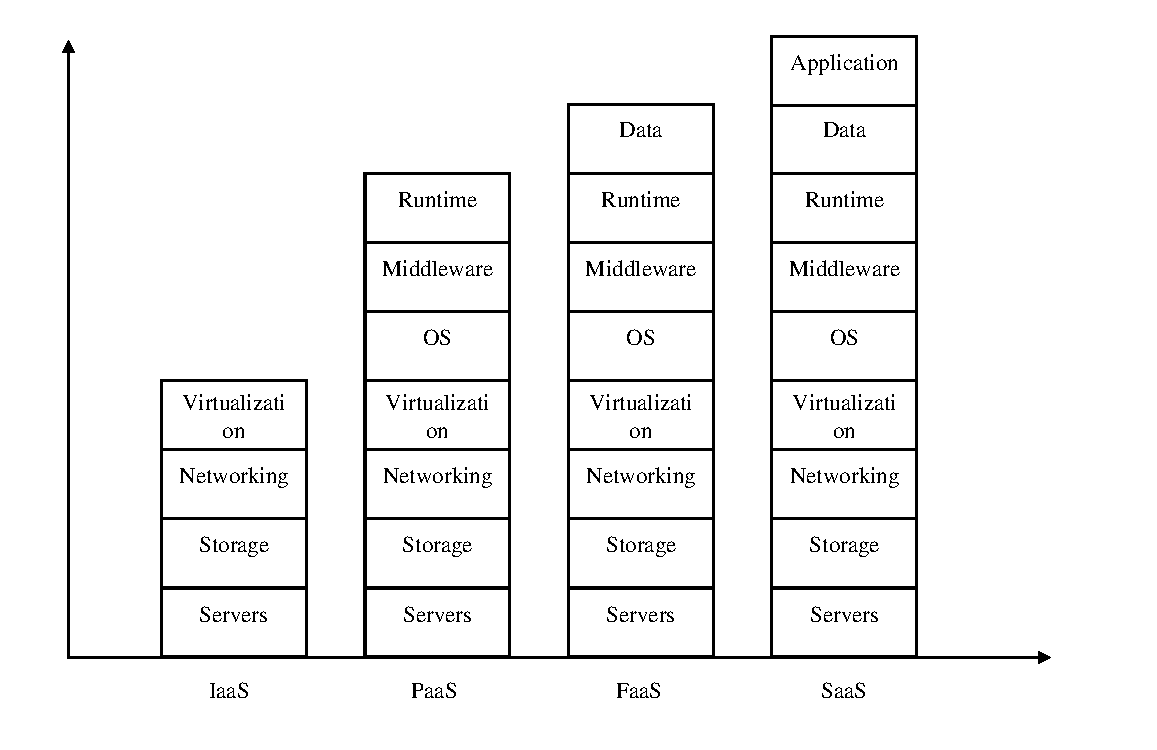
\includegraphics[width=0.9\columnwidth]{2_grundlagen/vergleich-service-modelle.pdf}
  \caption{Vergleich der Elemente von Service-Modellen \autocite{jiang2020overview}}
  \label{Kap2:VergleichServiceModelleElemente}
\end{figure}

\autoref{Kap2:VergleichServiceModelleElemente} vergleicht die Service-Modelle ebenfalls uns zeigt auf, welche Elemente von welchem Modell geliefert werden. Dabei ist auffällig, dass von links nach rechts mehr Elemente bereitgestellt werden. Für die Neuentwicklung von Anwendungen bedeutet das, dass \ac{FaaS} und \ac{BaaS} geeignet sind, da nur die Anwendungslogik geschrieben werden muss und die restlichen Elemente vom Anbieter selbst kommen.

\section{Anbieter von \acl{BaaS}}

Im folgenden Abschnitt werden nun die für diese Arbeit relevanten Anbieter von \ac{BaaS} vorgestellt. Außerdem wird eine Übersicht über weitere Anbieter gegeben.

\subsection{\acs{AWS} Amplify}

Da der Release von \ac{AWS} Amplify erst im November 2018 war, gibt es kaum wissenschaftliche Arbeiten, die sich mit \ac{AWS} Amplify selbst beschäftigen. Zur Erläuterung technischer Sachverhalte von \ac{AWS} Amplify eignet sich daher die offizielle Amplify Dokumentation \autocite{amplifyDocs}. Allerdings verbindet \ac{AWS} Amplify verschiedene Cloud-Dienste. Über diese Dienste lässt sich einiges an Literatur finden  \autocite{dahunsi2021commercial}\autocite{lysakov2021security}\autocite{mathew2014overview}\autocite{beach2014aws}.

Die offizielle Dokumentation beschreibt \ac{AWS} Amplify als eine Menge von Tools aus \ac{AWS} sowie Funktionalitäten, die Entwickler schnell und unkompliziert zusammenstecken können. Dies hat das Ziel, sowohl ein Backend als auch ein dazugehöriges Frontend in kürzester Zeit aufbauen und ausliefern zu können. Des Weiteren wird damit geworben, dass Entwickler keine Erfahrung im Bereich Cloud benötigen.

\ac{AWS} Amplify ist damit ein Wrapper um etliche \ac{AWS}-Dienste. Dieser Wrapper begünstigt den Einstieg in die Cloud-Dienste durch das Framework selbst. Die Libraries werden in Form von Quellcode zusammengefügt. Der Quellcode lässt sich über das Command-line Interface bedienen oder selbst anpassen. Werden zusätzliche Dienste benötigt, kann das auf Code-Level selbst oder über ein Custom Plugin geschehen, welches die nötigen Dienste erstellt.

Des Weiteren bietet \ac{AWS} Amplify ein Hosting des Frontends über CloudFront und S3 an. Alle Dienste werden in der \ac{AWS} CloudFormation als Stacks bereitgestellt. \ac{AWS} Amplify ist für die folgenden Plattformen geeignet:
\begin{itemize}
  \item Apple (iOS)
  \item Android
  \item Web
  \item React Native
\end{itemize}

In den nächsten Unterabschnitten werden die für diese Arbeit relevanten Amplify Libraries sowie weitere Libraries zusammengefasst dargestellt und erläutert.

\subsubsection{API (GraphQL)}

Mit dieser Library lassen sich GraphQL-Schnittstellen entwickeln. Der dahinterliegende Dienst ist \ac{AWS} AppSync. In jedem Fall wird eine Datenquelle benötigt, welche häufig die NoSQL-Datenbank Amazon DynamoDB ist. Wenn einzelne Queries oder Mutations Logik benötigen, dann besteht die Möglichkeit diese entweder mit der Programmiersprache VTL aufzulösen oder einen eigenen Resolver über \ac{AWS} Lambda hinzuzufügen. Weitere Funktionalitäten dieser Library sind die Authentifizierung über Amazon Cognito, \ac{AWS} IAM, einen API-Key oder eine eigene Lambda-Funktion. Auch Subscriptions bei definierten Events wie dem Erstellen, Aktualisieren oder Löschen eines Datensatzes sind möglich.

Für das Frontend besteht die Möglichkeit den Amplify GraphQL Client zu nutzen.

\subsubsection{Authentication}

Mit der Authentication-Library lassen sich sowohl für das Frontend als auch für das Backend Registrierung, Authentifizierung, Autorisierung und weitere Operationen abbilden. Im Backend wird dazu Amazon Cognito genutzt. Weitere Funktionalitäten dieses Dienstes sind Social Sign In (über Google, Facebook, Amazon und Apple), Multi-Factor Authentication, verschiedene Authentication-Abläufe sowie das Merken eines Geräts.

Im Frontend kann auf ein bereitgestelltes User Interface zurückgegriffen werden. Für weitere Anpassungen kann auch ein eigenes User Interface erstellt werden, was auf die selben Logik-Funktionen von Amplify zugreifen würde.

\subsubsection{Storage (S3)}

Mit der Storage-Library können Benutzerinhalte verwaltet werden. Im Backend wird dafür \ac{AWS} S3 verwendet, der als Speicherort für die Dateien dient. Im Standardfall wird der Bucket in einen öffentlichen, geschützten und privaten Bereich aufgeteilt. Auf den öffentlichen Bereich kann jeder Nutzer lesen und schreiben. Für den geschützten und privaten Bereich muss der Nutzer über \ac{AWS} Cognito eingeloggt sein. Beim geschützten Bereich kann nur der Besitzer schreiben, während alle anderen Nutzer lesen können. Im privaten Bereich kann nur der Benutzer lesen und schreiben. Wichtig ist zu erwähnen, dass die Identität und nicht die Benutzerkennung als Ordner-Pfad gesetzt werden. Dies benötigt eine Umrechnung, sollte eine Lambda-Funktion zu einem Nutzer den dazugehörigen Ordner finden wollen.

Im Frontend können die existierenden Funktionen von Amplify genutzt werden, um mit dem Storage zu agieren. Dabei werden in der Regel \textit{Signed URLs} verwendet.

\subsubsection{Weitere Libraries}

\ac{AWS} Amplify bietet eine Reihe weiterer Libraries, welche im folgenden kurz dargestellt werden.
\begin{itemize}
   \item \textit{API (\acs{REST})} wird genutzt, um \acs{REST}-APIs über den Dienst \ac{AWS} API Gateway abzubilden.
   \item \textit{Geo} wird genutzt, um APIs und User Interfaces für Karten und Standortsuchen über den \ac{AWS}-Dienst Amazon Location Service zu verwenden.
   \item \textit{DataStore} wird genutzt, um Daten mit einer Schnittstelle sowohl im Online- als auch im Offlinefall einheitlich über \ac{AWS} AppSync zu verwalten.
   \item \textit{Interactions} werden genutzt, um Chatbots über Amazon Lex in die Anwendung zu integrieren.
   \item \textit{Predictions} wird für gängige Aufgaben der künstlichen Intelligenz wie beispielsweise Übersetzungen, Text-to-Speach und Labelling genutzt. Dabei kommen die Dienste Amazon Translate, Amazon Polly, Amazon Transcribe, Amazon Rekognition, Amazon Textract, and Amazon Comprehend zum Einsatz.
   \item \textit{XR} wird für Augmented Reality and Virtual Reality genutzt.
\end{description}

\subsection{Firebase}

Firebase wurde im Jahr 2011 veröffentlicht und 2014 von Google übernommen. Im Gegensatz zu \ac{AWS} Amplify gibt es hier umfassende wissenschaftliche Literatur \autocite{moroney2017definitive}\autocite{tanna2018serverless}. Daneben bietet Firebase ebenfalls eine ausführliche Dokumentation\autocite{firebaseDocs} an.

Auch Firebase bietet etliche Libraries an, um Backend- und Frontendanwendungen zu entwickeln. Diese nutze teilweise auch andere Cloud-Dienste der Google Cloud Platform, andere sind wiederum direkt für Firebase geschrieben. Firebase ist für die Entwicklung auf den folgenden Plattformen geeignet:
\begin{itemize}
  \item Apple (iOS)
  \item Android
  \item Web
  \item C++
  \item Unity
\end{itemize}

\subsubsection{Cloud Functions}

Im Gegensatz zu \ac{AWS} Amplify gibt es hier keine GraphQL- oder Rest-Schnittstelle. Funktionen, auch \texti{Cloud Functions} genannt, werden stattdessen direkt aufgerufen. Diese können sowohl aus dem Frontend als auch durch eine Aktion im Backend aufgerufen werden. Ersteres erfordert die nötigen Berechtigungen für diese Funktion. Letzteres kann beispielsweise durch einen Trigger wie \texti{document.create} aus der Datenbank ausgelöst werden.

Für die Datenbank kann der Entwickler zwischen der Firestore Database und der Realtime Database wählen. Die Realtime Database ist die erste Version, während die Firestore Database eine schnellere und besser skalierbare Datenbank mit einem intuitiveren Datenmodell ist. Beide Datenbanken bieten entsprechende Frontend-Libraries an. Anders als in traditionellen Systemen besteht die Möglichkeit, dass das Frontend mit entsprechenden Berechtigungen ohne eine Funktion aufzurufen in die Datenbank schreiben kann. Die Sicherheitskonfiguration der Datenbank muss dafür so angepasst werden, dass Nutzer keine Datensätze anderer Nutzer überschreiben können.

\subsubsection{Authentication}

Auch Firebase bietet eine Authentication-Library für Frontend und Backend an. Diese funktioniert ähnlich wie die aus \ac{AWS} Amplify. Ebenfalls ist eine fertige Implementierung vorhanden. Auch hier können bei Bedarf eigene UI-Komponenten für Login, Registrierung und weitere Authentifizierungsdienste geschrieben werden. Der Social Sign-In ist über Google, Apple, Facebook, Twitter und GitHub möglich.

\subsubsection{Storage}

Auch die Storage-Library unterscheidet sich für den einfachen Bedarf an benutzerspezifischen Inhalten kaum von \ac{AWS} Amplify. Im Hintergrund wird der Cloud Storage-Dienst genutzt. Das Berechtigungssystem wird bei diesem Dienst über Regeln definiert, welche eine Konfigurationsdatei darstellen. Diese Regeln können auch an das Authentication-System geknüpft sein, um einen privaten Benutzerbereich zu schaffen.

\subsubsection{Weitere Libraries}

Firebase bietet zudem eine Menge an weiteren Libraries.

\begin{itemize}
  \item \textit{Cloud Messaging} wird genutzt, um Push-Notifiations abzubilden.
  \item \textit{Firebase ML} wird für Text-, Bild-, Gesichts und Objekterkennung sowie Übersetzungen, intelligenten Antworten oder Barcode-Scans genutzt.
  \item \textit{Google Analytics} wird zum Tracking von Userverhalten genutzt.
  \item \textit{Remote Config} wird genutzt, um Verhalten mit Feature-Flags zu ändern und zu testen.
  \item \textit{Performance Monitoring} wird zum Überwachen der Latenzzeiten genutzt.
  \item \textit{Test Lab} wird zum Testen der Anwendung auf verschiedenen Endgeräten genutzt.
\end{description}

Zusätzlich gibt es bei Firebase eine Menge Extensions, um das System schnell zu erweitern. Beispiele dafür sind Payment-Anbindungen, Bildbearbeitungstools oder ein URL-Shortener.

\subsection{Weitere Anbieter}